\documentclass[sigconf,natbib=true,anonymous=true]{acmart}
\settopmatter{printacmref=false}
% Review submission: do not pre-populate proceedings or rights metadata.
\usepackage{booktabs}
\usepackage{tikz}
\usetikzlibrary{arrows.meta,positioning}
\title{Reproducibility Audit of a News Event-Clustering System: Dataset Provenance, Decision Logic, and Evaluation Traceability}
\begin{CCSXML}
<ccs2012>
 <concept>
  <concept_id>10002951.10003317.10003347</concept_id>
  <concept_desc>Information systems~Document representation</concept_desc>
  <concept_significance>500</concept_significance>
 </concept>
 <concept>
  <concept_id>10010147.10010257.10010258.10010260</concept_id>
  <concept_desc>Computing methodologies~Natural language processing</concept_desc>
  <concept_significance>300</concept_significance>
 </concept>
 <concept>
  <concept_id>10002951.10003317.10003359</concept_id>
  <concept_desc>Information systems~Clustering</concept_desc>
  <concept_significance>300</concept_significance>
 </concept>
</ccs2012>
\end{CCSXML}
\ccsdesc[500]{Information systems~Document representation}
\ccsdesc[300]{Computing methodologies~Natural language processing}
\ccsdesc[300]{Information systems~Clustering}
\begin{document}
\begin{abstract}
Reliable evaluation of news-event clustering requires the evaluated implementation, benchmark provenance, labels, model configuration, and per-pair predictions to be traceable. This paper presents a reproducibility audit of a news aggregation system whose event-matching component combines unigram Jaccardrdrd similarity, character 3-gram cosine similarity, a five-signal Enhanced Fusion Scoring Algorithm (EFSA), and selective large language model (LLM) verification. A read-only audit of repository artifacts covering 5,000 benchmark records found that all records contain two identical annotation fields, but the repository does not establish that these labels were independently produced; 4,755 records are flagged by note-pattern heuristics as programmatic or structured extensions. The audit also identifies incompatible evaluation partitions, a simulated perfect-classifier result, and an evaluation script that does not execute the complete cascade. The production decision rule is an OR gate across Jaccard, character cosine, and EFSA thresholds, contrary to a sequential cascade described in earlier drafts. Consequently, existing accuracy, call-reduction, cost, and latency values are not treated as validated comparative findings. The contribution is a documented audit method, quantified provenance findings, and a reproducible protocol for a future controlled evaluation.
\end{abstract}
\keywords{news aggregation, event clustering, candidate filtering, large language models, reproducibility, semantic similarity}
\maketitle

\section{Introduction}
% ============================================================

Automated news aggregation platforms must process continuous streams of articles, identifying when distinct journalistic outlets cover the same real-world incident.
For example, one wire service may headline ``Federal Reserve Lowers Benchmark Rate by 25 Basis Points,'' while another writes ``US Central Bank Cuts Borrowing Costs Amid Cooling Inflation.''
Despite sharing negligible surface token overlap, both headlines describe the exact same macroeconomic event.
Detecting this semantic equivalence is essential to organize incoming feeds into coherent event clusters, enabling users to examine diverse editorial perspectives without redundant coverage.

Event clustering on streaming text must balance computational cost against missed matches and incorrect merges:
\begin{enumerate}
    \item \textit{Lexical methods} (e.g., token Jaccard similarity or character $n$-grams) execute in microseconds but fail on synonymous phrasing, acronyms (``PBOC'' vs.\ ``People's Bank of China''), and entity aliasing (``Apple Inc.'' vs.\ ``Cupertino Giant'').
    \item \textit{Dense semantic embeddings} (e.g., Sentence-BERT~\cite{reimers2019sentence}) capture contextual similarity effectively, but pairwise vector distance comparisons over an active sliding window scale quadratically, straining unaccelerated CPU deployments.
    \item \textit{Generative LLMs} can be used as pairwise verifiers, but remote inference introduces per-call latency and potentially variable API cost.
\end{enumerate}

To describe the implementation accurately, The inspected implementation computes lexical similarity and EFSA signals for each recent event candidate. The configured LLM is called when any one of the candidate-gate conditions passes:
\begin{itemize}
    \item \textbf{Candidate gate.} The implementation calculates unigram Jaccard similarity and character 3-gram cosine similarity for each recent event candidate.
    \item \textbf{Evidence fusion.} EFSA combines keyword overlap, character 3-gram cosine, rule-based entity overlap, temporal decay, and sector evidence.
    \item \textbf{Selective LLM verification.} The current implementation calls the configured Groq model when Jaccard, character 3-gram cosine, or EFSA reaches its respective threshold.
\end{itemize}

The contributions are threefold: a code-grounded description of the event-matching decision path; a reproducibility audit of benchmark and result artifacts; and a concrete protocol for evaluating candidate filtering without conflating generated stress cases, independently labeled examples, simulated outputs, and measured inference traces. The work does not claim that the audited system outperforms existing methods.

% ============================================================
\section{Related Work}
% ============================================================

\subsection{Lexical Similarity and Event Matching}
Classical information retrieval uses term weighting and lexical overlap to rank or compare text~\cite{salton1988,aggarwal2012}. Such methods are computationally inexpensive, but surface-form overlap may be insufficient when headlines describe the same occurrence using different wording. News-event clustering must distinguish topical similarity from event identity: two articles can mention the same organization without reporting the same incident.

\subsection{Sentence Representations and Pairwise Matching}

Sentence-BERT maps sentences into dense vector representations for semantic similarity comparison~\cite{reimers2019sentence}. Pairwise matching has also been studied using pre-trained language models, including the Ditto entity-matching framework~\cite{li2020ditto}.
The repository also contains an offline SBERT evaluation path, but it is not invoked by the inspected production event-matching module.

\subsection{LLM Verification and Gated Cascades}
Surveys of large language models discuss capabilities and deployment considerations across a broad range of tasks~\cite{zhao2023}. For cost-aware event matching, the relevant empirical question is how candidate filtering changes call volume, false-negative coverage, latency, and measured cost. Those outcomes require a common, independently labeled benchmark; this draft does not claim that the current implementation outperforms alternatives.

% ============================================================
\section{System Under Audit}
% ============================================================

\begin{figure}[!t]
\centering
\resizebox{\columnwidth}{!}{%
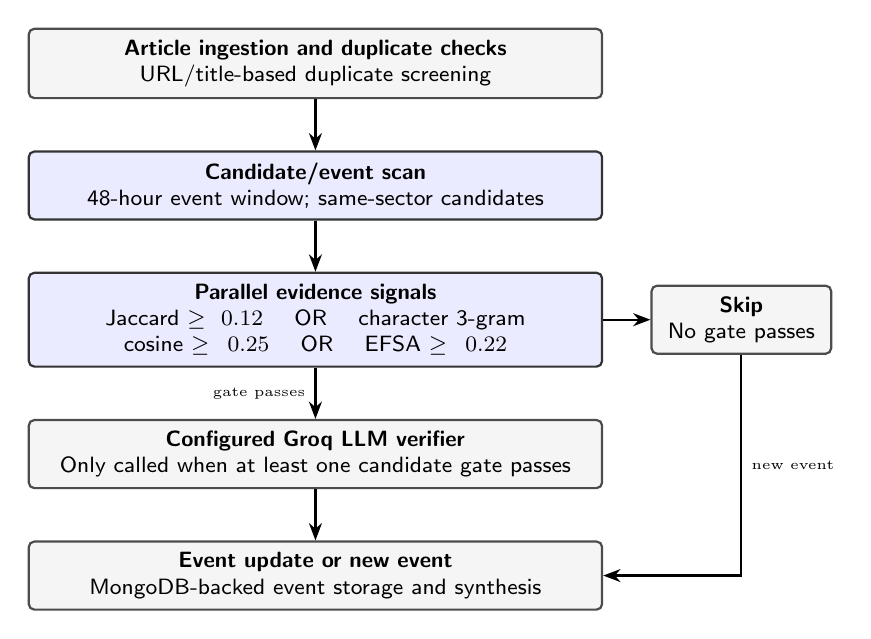
\begin{tikzpicture}[
    node distance=0.65cm,
    font=\sffamily\footnotesize,
    box/.style={rectangle, draw=black!70, thick, rounded corners=2pt, align=center, minimum height=0.65cm, inner sep=4pt, fill=black!4},
    gate/.style={rectangle, draw=black!80, thick, rounded corners=2pt, align=center, minimum height=0.75cm, inner sep=4pt, fill=blue!8},
    arrow/.style={-{Stealth[length=2.2mm]}, thick}
]
\node[box, text width=7.0cm] (ingest) {\textbf{Article ingestion and duplicate checks}\\URL/title-based duplicate screening};
\node[gate, below=of ingest, text width=7.0cm] (candidate) {\textbf{Candidate/event scan}\\48-hour event window; same-sector candidates};
\node[gate, below=of candidate, text width=7.0cm] (signals) {\textbf{Parallel evidence signals}\\Jaccard $\geq 0.12$ \quad OR \quad character 3-gram cosine $\geq 0.25$ \quad OR \quad EFSA $\geq 0.22$};
\node[box, below=of signals, text width=7.0cm] (llm) {\textbf{Configured Groq LLM verifier}\\Only called when at least one candidate gate passes};
\node[box, below=of llm, text width=7.0cm] (store) {\textbf{Event update or new event}\\MongoDB-backed event storage and synthesis};
\node[box, right=0.6cm of signals, text width=2.0cm] (skip) {\textbf{Skip}\\No gate passes};
\draw[arrow] (signals.east) -- (skip.west);
\draw[arrow] (ingest) -- (candidate);
\draw[arrow] (candidate) -- (signals);
\draw[arrow] (signals) -- node[left,font=\tiny]{gate passes} (llm);
\draw[arrow] (llm) -- (store);
\draw[arrow] (skip.south) |- node[pos=0.25,right,font=\tiny]{new event} (store.east);
\end{tikzpicture}%
}
\caption{Decision path reflected in the current event-matching implementation. The lexical and EFSA conditions act as an OR gate; EFSA is not a mandatory sequential stage after the lexical filters.}
\label{fig:architecture}
\end{figure}

\subsection{Pipeline Overview}
The repository documentation reports different feed counts in different locations; the exact feed inventory and sector count should be frozen from the deployment configuration before submission.
Incoming articles are pre-screened for exact duplicates using URL hashing and MD5 title signatures:
$\text{Match} = (\text{url} = U) \lor (\text{MD5}(T_1) = \text{MD5}(T_2))$.
Unique articles are evaluated against active event clusters initiated within the previous 48 hours.
The multi-tier filtering topology is depicted in Fig.~\ref{fig:architecture}.

\subsection{Candidate Filtering}
For each recent event in the 48-hour window and matching sector, the implementation calculates unigram Jaccard similarity and character 3-gram cosine similarity. The configured thresholds are $\tau_J=0.12$ and $\tau_C=0.25$. The code uses these metrics alongside EFSA to decide whether an LLM verification call is warranted.

\subsection{Enhanced Fusion Scoring Algorithm (EFSA)}
For each candidate event, EFSA combines five heterogeneous evidence channels into a scalar score:
\begin{equation}
S_{\text{EFSA}}(A, B) = \sum_{i=1}^{5} w_i S_i(A, B)
\label{eq:efsa}
\end{equation}
The component signals $S_i$ and configured weights $w_i$, which sum to 1.00 in the current implementation, are defined as:
\begin{itemize}
    \item $S_{\text{key}}$ ($w_1 = 0.25$): Keyword intersection-over-union after English stopword removal.
    \item $S_{\text{head}}$ ($w_2 = 0.30$): Character 3-gram cosine similarity between headline strings.
    \item $S_{\text{ent}}$ ($w_3 = 0.25$): Entity overlap ratio $J_{\text{ent}} = |E_A \cap E_B| / |E_A \cup E_B|$, where entity candidates are extracted with a capitalization- and number-based regular expression.
    \item $S_{\text{temp}}$ ($w_4 = 0.10$): Exponential temporal decay $S_{\text{temp}} = e^{-\lambda \Delta t}$, where $\Delta t$ is publication delta in hours and $\lambda = 0.02$.
    \item $S_{\text{sec}}$ ($w_5 = 0.10$): Sector taxonomy match indicator (1.0 for matching sectors, 0.5 otherwise).
\end{itemize}

\subsection{Selective LLM Verification}
The current implementation calls the verifier when any of the following conditions is true:
\begin{equation}
(J \geq \tau_J) \lor (C \geq \tau_C) \lor (S_{\text{EFSA}} \geq \tau_{\text{EFSA}}).
\label{eq:decision}
\end{equation}
The thresholds in the repository are $\tau_J=0.12$, $\tau_C=0.25$, and $\tau_{\text{EFSA}}=0.22$. The model identifier is configurable through the \texttt{GROQ\_MODEL} environment variable; the code fallback currently names \texttt{openai/gpt-oss-120b}. The exact deployed model must be established from deployment configuration or request logs, not inferred from older comments or README text. The verifier compares two headlines and returns a SAME/DIFFERENT decision. The implementation returns false on API failure, which should be included in reliability evaluation.

\subsection{Embedding Baseline}
The repository contains SBERT evaluation scripts and result files, but the active event-matching path inspected for this audit does not invoke the ONNX/SBERT fallback. SBERT is therefore treated as an offline baseline, not as a production stage in the architecture.

% ============================================================
\section{Audit Method and Data Sources}
% ============================================================

\subsection{Implementation Configuration and Telemetry}
The repository implements a Node.js event-processing backend using Express and MongoDB, with Groq API calls configured through environment variables. The deployment provider, instance size, exact package versions, database indexes, and production configuration must be verified from deployment records before they are reported as experimental setup. The repository contains an in-memory AI telemetry utility that accumulates call counts, token counts, model names, and inference latency during a process lifetime, with a rolling window of recent call latencies. The inspected telemetry utility does not itself establish a persisted 30-day record or an end-to-end ingestion latency distribution. Production-volume, webhook, and latency figures are therefore omitted from quantitative claims in this revision until timestamped logs or a persisted telemetry export can be archived and independently checked.

\begin{table}[!t]
\centering
\caption{Technology Stack Identified in the Repository}
\label{tab:tech}
\resizebox{\columnwidth}{!}{%
\begin{tabular}{lll}
\toprule
\textbf{Component} & \textbf{Technology} & \textbf{Function} \\
\midrule
Runtime & Node.js & Async pipeline orchestration \\
Web Framework & Express.js & REST API and webhook routing \\
Database & MongoDB Atlas & Article metadata \& event store \\
LLM Inference & Groq API (model configurable) & Candidate-pair verification \\
Offline baseline & SBERT evaluation scripts & Separate benchmark, not active event path \\
Frontend & React & Admin monitoring dashboard \\
\bottomrule
\end{tabular}%
}
\end{table}

\subsection{Benchmark Provenance and Split Integrity}
The repository contains multiple evaluation artifacts that must not be treated as one experiment. One reported partition uses 519 training, 166 validation, and 198 test pairs, while a separate split report records 2,990 training, 988 validation, and 1,022 test pairs from a 5,000-item dataset. The 883-pair builder imports a synthetic template generator and populates annotator fields from expected labels for at least part of the data. Some split records are explicitly marked as programmatic or structured extensions. A separate inter-annotator agreement report describes 250 pairs from \texttt{testCases\_v2\_real.json}; that result does not establish independent annotation of every pair in the 883-item benchmark. These artifacts require provenance review before their labels can support a held-out performance claim. The audit summary is shown in Table~\ref{tab:split-audit}.

\begin{table}[!t]
\centering
\caption{Repository Audit of the 5,000-Record Dataset}
\label{tab:split-audit}
\resizebox{\columnwidth}{!}{%
\begin{tabular}{lrrrr}
\toprule
\textbf{Split} & \textbf{Records} & \textbf{Flagged notes} & \textbf{Matching labels} & \textbf{Duplicate pairs} \\
\midrule
Train & 2,990 & 2,808 & 2,990/2,990 & 0 \\
Validation & 988 & 954 & 988/988 & 0 \\
Test & 1,022 & 993 & 1,022/1,022 & 0 \\
\midrule
Total & 5,000 & 4,755 & 5,000/5,000 & 0 \\
\bottomrule
\end{tabular}%
}
\end{table}

A reproducible evaluation should freeze exact pair IDs and labels; publish dataset and split hashes; identify the source and date for each headline; record independent annotator labels and adjudication; and ensure that thresholds are selected on training/validation data only. The held-out test set must be evaluated only after the model, thresholds, and implementation commit are frozen.

% ============================================================
\section{Audit Results and Evaluation Protocol}
% ============================================================

\subsection{Status of Quantitative Claims}
The audit identified several distinct evaluation records. One result file reports a 198-pair configuration with $TP=25$, $FP=0$, $TN=99$, and $FN=74$, corresponding to 62.63\% accuracy, 100\% precision, 25.25\% recall, and 40.32\% F1 when those counts are taken at face value. These are artifact-reported values only; the audit did not establish that their predictions were generated by a reproducible run on independently validated labels. A separate evaluation artifact uses a different class balance ($157$ positive and $41$ negative pairs) and explicitly states that LLM calls were simulated as a perfect classifier. The script \texttt{runCascadeOnTestSet.js} reads an existing result file and prints stage counts as \texttt{TBD}; it does not execute the full cascade. Therefore, neither call reduction nor the simulated LLM-only result is accepted as a measured comparative finding.

The active event-matching code also differs from the sequential architecture used in earlier manuscript drafts: the LLM is triggered by an OR of the Jaccard, character cosine, and EFSA conditions. In addition, the model fallback in the active event engine is \texttt{openai/gpt-oss-120b}, while the telemetry utility has a different fallback identifier. The exact deployed model must be recovered from deployment configuration and actual request traces before reporting model-specific accuracy, latency, or cost.

Accordingly, no comparative accuracy, precision, recall, F1, call-reduction, cost, or production-latency values are asserted here as validated results. This is an explicit evidence limitation, not a claim that the system has no useful performance. A submission-ready empirical version requires rerunning each baseline and the implemented candidate gate against the same frozen, independently adjudicated test pairs and saving per-pair predictions, actual LLM responses, stage counts, timing boundaries, token usage, and configuration metadata.

\subsection{Economic Cost Analysis}
A cost estimate should be computed from the model and prices actually active during the measured experiment, along with observed prompt and completion token counts. A generic estimate can be calculated as
\begin{equation}
C = \frac{N_{\mathrm{in}}P_{\mathrm{in}}+N_{\mathrm{out}}P_{\mathrm{out}}}{10^6},
\label{eq:cost}
\end{equation}
where $N_{\mathrm{in}}$ and $N_{\mathrm{out}}$ are measured input and output tokens and $P_{\mathrm{in}}$ and $P_{\mathrm{out}}$ are the applicable per-million-token prices. The current repository artifacts disagree on the cost per million comparisons and on the number of calls saved; no absolute operating-cost or percentage-saving claim is therefore made in this revision.

\subsection{Dynamic Publisher Credibility Scoring (DPCS)}
The repository includes a DPCS component and result artifacts describing experiments with publisher-consensus weighting. However, the present audit did not establish a single reproducible test run linking the reported accuracy values, statistical test, exact pair IDs, and active production configuration. DPCS is therefore described as an implemented or explored component, not as a statistically established negative result. A defensible comparison requires paired predictions from the same frozen test set and a prespecified statistical test.

\subsection{Limitations}
Two primary limitations should be noted.
First, the audit does not establish the independent origin or correctness of all benchmark labels, and the note-pattern heuristic may over-flag curated records or fail to identify generated examples without notes. Second, the audit inspects repository artifacts rather than reproducing production deployment conditions; it does not establish deployed model identity, end-to-end latency, or actual API cost. Third, the system description is limited to the inspected code path and does not establish generalization to multilingual news streams.

% ============================================================
\section{Future Work}
A follow-up study should establish a source-traceable corpus, independently annotate and adjudicate a frozen test set, and release privacy- and copyright-compliant pair identifiers with dataset hashes and annotation instructions. The evaluation harness should execute the committed decision path rather than read precomputed summaries, record a prediction and stage trace for every pair, and compare lexical, EFSA, embedding, and actual LLM-based methods on identical held-out examples. Model identifiers, prompts, thresholds, API failures, token usage, latency boundaries, and applicable prices should be fixed or logged before the run; uncertainty estimates and paired significance tests should be computed from the resulting predictions. Any generated examples should be reported separately as stress tests, and the manuscript should be updated only from archived artifacts that can be independently reproduced.\n\n\section{Conclusion}
% ============================================================

This paper presented a repository-level reproducibility audit of a news event-matching component. The audit documents an OR-connected candidate gate and identifies limitations in benchmark provenance, annotation independence, result consistency, simulated model outputs, and execution traces. The findings do not establish that the event matcher lacks utility; they establish that the current artifacts are insufficient for defensible comparative performance claims. The next step is a frozen, independently adjudicated benchmark, followed by rerunning the actual implementation and every baseline under identical conditions. Accuracy, cost reduction, confidence intervals, and latency should be reported only from those traceable runs.

% ============================================================
\begin{thebibliography}{99}
\footnotesize
\setlength{\itemsep}{1pt}
\setlength{\parskip}{0pt}

\bibitem{aggarwal2012}
C.~C.~Aggarwal and C.~Zhai, ``A survey of text clustering algorithms,'' in \textit{Mining Text Data}, Springer, 2012, pp.\ 77--128.

\bibitem{li2020ditto}
Y.~Li, J.~Li, Y.~Suhara, A.~Doan, and W.-C.~Tan, ``Deep entity matching with pre-trained language models,'' \textit{Proc. VLDB Endowment}, vol.~14, no.~1, pp.~50--60, 2020, doi: 10.14778/3421424.3421431.

\bibitem{reimers2019sentence}
N.~Reimers and I.~Gurevych, ``Sentence-BERT: Sentence embeddings using Siamese BERT-networks,'' in \textit{Proc.\ 2019 Conf. Empirical Methods Natural Lang. Process. 9th Int. Joint Conf. Natural Lang. Process. (EMNLP-IJCNLP)}, Hong Kong, China, 2019, pp.\ 3982--3992.

\bibitem{salton1988}
G.~Salton and C.~Buckley, ``Term-weighting approaches in automatic text retrieval,'' \textit{Inf. Process. Manage.}, vol.~24, no.~5, pp.\ 513--523, 1988.

\bibitem{zhao2023}
W.~X.~Zhao \textit{et al.}, ``A survey of large language models,'' \textit{arXiv preprint arXiv:2303.18223}, 2023.

\end{thebibliography}

\end{document}
